% vim: set spelllang=fr:

\setchapterpreamble[ur][\textwidth]{%
  \dictum[Bill Watterson, \textit{Calvin et Hobbes}]{%
    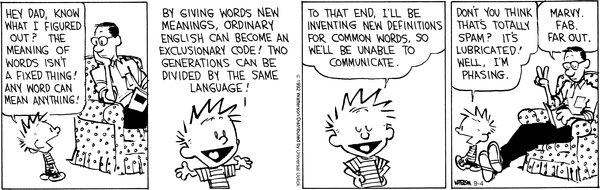
\includegraphics[width=\textwidth]{fig/calvin_meaning.png}}}

\chapter{Annotation en rôle sémantique en domaine spécifique}
\label{ch:domainsrl}

\section{Introduction}

Là où le précédent chapitre présentait sur l'annotation en rôles sémantiques
fondée sur la connaissance, celui-là se concentre sur l'annotation en domaines
spécifiques. À l'heure où les algorithmes supervisés obtiennent d'excellentes
performances sur un certain nombre de tâche, l'adaptation au domaine est un
défi majeur du Traitement Automatique des Langues, et l'annotation en rôles
sémantiques sur de nouveaux domaines reste un problème ouvert. 
% TODO existing approaches ici ?

Nous présentons dans ce chapitre un système d'annotation en rôles sémantiques
qui n'utilise que la ressource VerbNet (présentée à la
section~\ref{presentation_verbnet}), ce qui rend la méthode applicable
dans toute langue disposant d'un VerbNet, ce qui est le cas par exemple de
l'Estonien \citep{jentson2014verbnet}, du français (Chapitre~\ref{ch:verbnet})
ou du Portuguais \citep{scarton2012towards}, entre autres. L'approche ne dépend
pas du domaine étant donné que VerbNet couvre l'ensemble des verbes du
vocabulaires\footnote{La plupart des erreurs liées à VerbNet sont un manque
général, et non pas spécifique au domaine étudié
(section~\ref{sec:enrichissement_verbnet}).}. L'approche est aussi facile à
reproduire en raison de sa simplicité : les arguments du verbe sont simplement
mis en correspondance avec VerbNet. Notre système est donc suivant le point de
vue une \emph{baseline} forte, une première étape pour annoter un nouveau
domaine avec peu d'efforts, ou la base d'un système complet d'annotation en
rôles sémantiques une fois que VerbNet a été mis à jour par rapport au domaine.
De plus, cette méthode peut identifier des manquements dans VerbNet.

La définition du terme 'domaine' reste assez vague dans le sens où il est
difficile de proposer une catégorisation de la connaissance en un ensemble de
domaines qui soit à la fois cohérente et efficace pour le Traitement
Automatique des Langues. Il est aussi difficile de séparer clairement le
«~domaine général~» des domaines spécifiques. Néanmoins, c'est un phénomène qui
existe et qui est à considérer : les modèles entraînés sur un corpus d'un
domaine spécifique (la finance par exemple) généraliseront mal à d'autres
domaines (le football).


% TODO wordnet domains issues ma2012rethinking

% TODO proof with existing system? cite paper?

Il est important aussi de différencier le genre et le domaine d'un texte. Le
corpus du Wall Street Journal traite du domaine de la finance dans un genre
journalistique. D'autres genres existent, par exemple les genre littéraires que
sont la fiction, la poésie, le théâtre, etc. Néanmoins, ces distinctions ne
nous concernent pas ici, et l'objectif affiché est de traiter aussi bien un
roman qu'une encyclopédie qu'un email bien écrit qu'un article de journal.
C'est une simplification mais les difficultés que nous rencontrons avec les
corpus utilisés dépendent plutôt du domaine que du genre. En effet, dans deux
domaines différents plus que dans deux genres différents, les changements vont
résider dans les verbes utilisés, leur sens et la façon de les utiliser. C'est
ce que nous souhaitons prendre en compte ici.

\section{Travaux existants}

SEMAFOR \citep{das2014frame} est le système supervisé le plus proche de notre
système. En utilisant le corpus FrameNet, il commence par identifier les
prédicats, puis identifie la frame correcte évoquée par ces prédicats, puis
identifie les groupes de mots qui jouent un rôle pour ce prédicat donné.

% TODO compréhension située ?
% TODO mieux identifier ce que cette tâche fati
\cite{chen2008learning} entraînent un système de commentaires à partir de
commentaires existants et d'états de simulations de parties de football, mais
sans connaissance explicite de l'anglais. Leur approche a inspiré d'autres
travaux sur la compréhension située de la langue : \citep{bordes2010towards} et
\cite{richardson2012towards} ont proposé par la suite d'autres corpus pour
entraîner de tels systèmes. Notre système est similaire dans le sens où nous
minimisons l'effort humain pour annoter automatiquement de nouveaux domaines,
mais nous nous concentrons sur la tâche de l'annotation en rôles sémantiques de
type FrameNet.

Le système d'annotation en rôles sémantiques de \cite{gormley2014low} ne
demande certes pas de syntaxe supervisée, mais nécessite tout de même un corpus
annoté en rôles sémantiques. \cite{hadouche2011annotation} réalise de
l'annotation en rôles sémantiques sur un de nos trois corpus (DicoInfo) avec
deux approches différentes :

\begin{itemize}

    \item en appliquant des règles définies manuellement à la sortie d'un
        analyseur syntaxique

    \item en apprenant un système supervisé avec différents traits issus de la
        littérature

\end{itemize}

Nos travaux vont dans la direction opposée : nous annoter un grand nombre de
phrases provenant de divers domaines sans utiliser de corpus annoté.

\section{Approche}

Nous laissons ici l'identification des arguments à un travail futur, et
utilisons ici les arguments dits gold : on sait que ces arguments jouent un
rôle, mais on ne sait pas lequel. La raison est que nous voulons nous
concentrer pour le moment sur la capacité qu'à VerbNet à annoter des corpus à
la façon FrameNet sans avoir à analyser syntaxiquement notre corpus, ce qui
représente une difficulté supplémentaire. Cela signifie aussi que nous
n'évaluons pas l'identification des arguments jouant un rôle, ce qui est une
part importante de tout système d'annotation en rôles sémantiques.

Pour annoter une phrase donnée avec des remplisseurs de rôle déjà identifiés
(mais pas la classe ni les rôles), nous listons d'abord toutes les classes qui
peuvent être déclenchées par un verbe donné. Par exemple, étant donné la phrase
\emph{The online judge allocates the same amount of memory to both chess
engines}, la seule classe possible pour le verbe \emph{allocate} est
\texttt{future\_having-13.3}. Dans d'autres cas, le choix pourrait être ambigu.
C'est le cas notamment de \emph{The ocean circulation transports warm water to
the North Atlantic} : les deux classes \texttt{amuse-31.1} et
\texttt{send-11.1} sont possibles pour le verbe \emph{transport}.

Maintenant qu'une liste de classes a été établie, la phrase est représentée
avec la notation Verbnet, qui est par exemple \texttt{NP} \texttt{V}
\texttt{NP} \texttt{\{to\}} \texttt{PP} pour nos deux phrases d'exemples.

Ensuite, de simple transformations permettent de gérer l'encodage spécifique de
frames dans DicoInfo et DicoEnviro pour l'adapter à VerbNet. Premièrement, des
rôles répétés sont supprimés : \texttt{NP.Agent} \texttt{V} \texttt{NP.Theme}
\texttt{NP.Theme} devient \texttt{NP.Agent} \texttt{V} \texttt{NP.Theme}. En
effet, DicoInfo et DicoEnviro répètent le même rôle deux fois quand deux
syntagmes nominaux liés par exemple avec la conjonction \emph{et} partagent le
même rôle dans la même frame. Deuxièmement, au moment de rencontrer une forme
\texttt{V} \texttt{NP.Theme}, le syntagme devant le verbe est aussi supprimé
dans VerbNet avant comparaison. Ces formes sont en général des verbes à
l'impératif où le sujet n'est pas exprimé, et doivent dont êtres transformées
avant traitement par VerbNet, VerbNet ne décrivant les frames qu'à l'indicatif.
% TODO linguistique de collège ?

La phrase transformée est ensuite comparée aux frames VerbNet possibles dans
les classes candidates. Pour la première phrase, la seule option possible est
\texttt{NP.Agent} \texttt{V} \texttt{NP.Theme} \texttt{\{to\}} \texttt{PP.Goal}
(\textit{We offered our paycheck to her}) de la classe
\texttt{future\_having-13.3}. Pour la deuxième phrase, la seule option possible
est \texttt{NP.Agent} \texttt{V} \texttt{NP.Theme} \texttt{\{to\}}
\texttt{PP.Destination} dans la classe \texttt{send-11.1}. La prise en compte
des cadres de sous-catégorisation des frames VerbNet permet non seulement
d'identifier la classe correcte mais aussi d'assigner des rôles sémantiques aux
remplisseurs de rôle.

Deux difficultés peuvent se poser au momant de réaliser cette correspondance :
\begin{itemize}

    \item la frame n'est présente dans aucune classe VerbNet : c'est un
        manquement dans VerbNet

    \item la frame seule ne permet pas de désambiguïser entre différentes
        classes et donc différents rôles, le sens du rôle dépendant de la
        classe

\end{itemize}
        
Notre approche est trop simple pour gérer la deuxième difficulté, mais elle
permet de soulever des erreurs dans VerbNet lors de la première erreur
(section~\ref{sec:enrichissement_verbnet}). Le résultat de notre algorithme
est que chaque prédicat est potentiellement associé à une classe Verbnet, et
chaque argument issu de la vérité-terrain est potentiellement associé à un rôle
sémantique.

\section{Enrichissement de VerbNet}
\label{sec:enrichissement_verbnet}

Malgré leur similarité, ces corpus posent des problèmes différents vis-à-vis de
leur annotation avec VerbNet, tous liés au fait de ne pas être dans le "domaine
général". Nous avons considéré comme problème les manquements dans VerbNet qui
empêchent de prendre en compte les phrases considérées, indépendamment de
l'algorithme. Ainsi, pour que VerbNet puisse prendre en compte une instance, il
faut :

\begin{itemize}
    \item que le sens du verbe considéré soit présent dans VerbNet,
    \item que la construction en question soit présente dans VerbNet,
    \item et que les rôles sémantiques associés à chaque syntagme soient correct.
\end{itemize}

Il y a différentes façons de ne pas respecter ces contraintes :

\begin{itemize}
    \item Le verbe n'existe pas du tout dans VerbNet
    \item Le sens du verbe utilisé n'est pas représenté dans VerbNet alors que c'est un sens du domaine général
    \item Le sens du verbe utilisé n'est pas représenté dans VerbNet alors que c'est un sens spécifique à ce domaine
    \item La construction utilisée n'est pas présente dans VerbNet
    \item La construction utilisée est incorrecte dans VerbNet
\end{itemize}

Suivant les corpus considérés, les proportions d'erreurs seront différentes.
Nous avons demandé à deux annotateurs d'évaluer, pour vingt phrases par
domaine, quelle était l'erreur. L'accord inter-annotateur permet de valider la
distinction domaine spécifique/domaine général malgré l'impossibilité de la
définir précisément. % TODO lefaire

C'est pour cette raison que l'enrichissement de VerbNet se fait de deux
manières : certains verbes et constructions sont ajoutés comme faisant partie
du domaine général, alors que d'autres sont étiquetés avec le domaine
spécifique correspondant. L'idée est d'éviter que des connaissances de domaines
spécifiques viennent réduire la qualité de la ressource tout en s'assurant que
la couverture de VerbNet pour le domaine général continue de s'améliorer.

\section{Détection semi-automatique d'erreurs}

D'une part, pour minimiser le travail manuel, il est important d'automatiser au
maximum l'enrichissement de la ressource. D'autre part, l'intérêt de VerbNet
réside notamment dans sa capacité à factoriser efficacement ces informations
sur l'interface syntaxico-sémantique d'un verbe donné, et il est donc possible
et utile de valider manuellement chacun des changements apportés.

Le principe suivi est donc d'essayer de détecter les manquements de VerbNet de
manière automatique avant de proposer à un utilisateur expert de réaliser des
changements en ayant un maximum d'informations pertinentes à portée de main.

Les différentes erreurs détectées sont :
\begin{itemize}
    \item l'absence de lemmes dans la ressource
    \item l'absence d'un sens correct dans la ressource
    \item l'absence de constructions correctes dans la ressource
    \item l'absence de mapping de role correct dans la ressource
\end{itemize}

Nous avons d'abord commencé par détecter l'absence de constructions correctes,
ce qui a permis ensuite de détecter une absence de sens en comparant les
constructions observées avec les constructions présentes. Enfin, cela a permis
de faire des propositions quant à la position d'un nouveau lexème dans la
ressource.

\section{Expériences}


\subsection{Corpus considérés}

Afin de s'assurer que notre travail reste valide en changeant de domaine, nous
considérons ici trois corpus présents dans des domaines différents.

\begin{itemize}

    \item le Kicktionary \citep{schmidt2009kicktionary} rassemblant des
        dépêches de l'UEFA dans le domaine du football à propos de la Ligue
        Europa, de la Champions League et de la Coupe du Monde. Ce corpus est
        disponible en français, anglais et allemand.

    \item Le DicoInfo est le corpus Informatique/Internet de l'OLST
        \citep{corpusolst} en anglais, français et espagnol.

    \item Le DicoEnviro est le corpus Réchauffement climatique de l'OLST
        \citep{corpusolst} en anglais, français et espagnol.

\end{itemize}

Les points communs majeurs de ces trois corpus sont :
\begin{enumerate}

    \item de s'inspirer librement de la théorie des Frame Semantics telle
        qu'elle est considérée dans FrameNet ce qui correspond aussi à une
        annotation VerbNet,

    \item d'être disponible à la fois en anglais et en français,

    \item d'être basés sur l'annotation dans un corpus d'un certain nombre de
        prédicats (ce n'est pas une annotation dite "full-text")

\end{enumerate}

Ce dernier point est plutôt un inconvénient : la manière la plus réaliste de
considérer un corpus d'entraînement est de réaliser une annotation dite
\textit{full-text} en annotant tous les prédicats rencontrés dans un texte
donné. Cependant, les contextes choisis dans DicoInfo et DicoEnviro l'ont été
sur des critères de diversité syntaxique. \citep{lhomme2012adding} Le postulat
que nous faisons dans ce travail est que notre méthode n'est pas affectée par
ce problème comme le serait un modèle statistique appris sur ces mêmes
contextes étant donné que la probabilité des différentes possibilités n'est pas
prise en compte.

Les trois corpus ont étés découpés en deux parties de taille égales : un corpus
d'entraînement et un corpus de test. Étant donné qu'il n'y a pas de modèle à
entraîner, ce corpus d'entraînement est simplement utilisé pour comprendre les
erreurs en l'analysant manuellement. Même si les trois corpus contiennent des
textes proches entre eux, ils sont issus de sources différentes et ont étés
écrits par des auteurs différents. Nous avons normalisé ces sources (par
exemple, DEBIAN2 et DEBIAN3 dans le corpus de l'OLST devient DEBIAN) et
utilisons cette information pour faire le découpage : une source spécifique ne
peut être présente que dans un ensemble. Le découpage résultant est disponible
avec le code source associé à ce chapitre.

\subsection{Mappings de rôles}

Ces trois corpus utilisent des rôles spécifiques. Les corpus DiCoInfo et
DicoEnviro utilisent les convetions VerbNet alors que le Kicktionary, qui suit
surtout FrameNet, définit un nouvel ensemble de rôle pour chaque frame, comme
\texttt{Passer}, \texttt{Moving\_Ball} ou \texttt{Shot}. Dans les trois cas,
les rôles ne correspondent pas directement aux rôles VerbNet, et il faut donc
établir une correspondance entre les rôles Verbnet les rôles des autres corpus.
Nous avons assigné manuellement une classe VerbNet à chaque classe des autres
corpus, tout en faisant correspondre les rôles. Le résultat de ce mapping est
disponible avec le code source associé à ce chapitre.

De plus, DicoInfo et DicoEnviro font une distinction entre les rôles core et
non core : nous n'avons annoté que les rôles core étant donné que VerbNet ne
considère que ces rôles, même si la distinction peut différer entre VerbNet et
DiCoInfo et DiCoEnviro. Étant donné qu'une frame DiCoInfo/DiCoEnviro est un
sens spécifique d'un verbe n'acceptant que des constructions spécifiques, nous
avons toujours mappé de tels sens vers une seule classe VerbNet.

Le Kicktionary a été plus difficile à mapper à VerbNet : ses frames considèrent
un grand nombre de verbes au comportement parfois assez différent. Les règles
de FrameNet indiquent que de telles frames auraient du êtres découpées
\citep{ruppenhofer2006extended}, mais le Kicktionary ne suit pas toujours ces
règles, ayant été développé à part de FrameNet. Certaines frames sont définies
correctement : c'est le cas de \texttt{Receive\_Card} et \texttt{Give\_Card}
qui correspondent respectivement à \texttt{obtain-13.5.2} et
\texttt{give-13.1-1}. Par contre, la frame \texttt{Goal} a par exemple été
définie pour un but marqué, mais les différentes façons de l'exprimer n'ont pas
étés séparées : ouvrir la marque, égaliser, frapper, et d'autres utiliseront
différentes constructions syntaxiques, évoquerons des rôles différents et
correspondront donc à des classes VerbNet différentes.

\section{Méthode d'évaluation}

Les trois corpus considérés ont été annotés en rôles sémantiques dans les deux
langues qui nous intéressent ici~: l'anglais et le français. Il nous suffit
donc d'utiliser un mapping entre les rôles considérés par ces ressources et les
rôles VerbNet avant d'évaluer la performance de l'algorithme basé sur la
connaissance d'annotation en rôles sémantiques présenté au
chapitre~\ref{ch:srl}.

Dans le cas de DicoInfo et DicoEnviro, les noms des rôles sont proches des noms
de rôles employée dans VerbNet et LIRICS \citep{bonial2011hierarchical} (Agent,
Patient, Destination, Instrument...). Cependant, même si les noms sont les
mêmes, la définition de ces rôles est spécifique à DicoInfo et DicoEnviro.
En pratique :

\begin{itemize}
    \item DicoInfo et DicoEnviro ne distinguent pas Theme de Patient mais
    n'utilise que Patient ce qui rend l'annotation plus facile.\footnote{La
    distinction entre Theme et Patient est difficile à établir. Dans \textit{Le
    chaton a léché mes doigts}, est-ce que mes doigts ont changé d'état ? Si oui,
    ils devraient être Patient, et sinon, Theme.\citep[p.~5]{palmer2010semantic}}
    \item Pour un certain nombre de lexies, la perspective du domaine implique
    souvent des rôles différents (TODO exemple Patient vs. Result) % TODO clair
\end{itemize}

C'est pour ces raisons que nous avons créé manuellement un mapping entre
VerbNet et les corpus considérés (DicoInfo et DicoEnviro). Ce mapping est
utilisé uniquement à des fins d'évaluation, et l'effort nécessaire pour le
créer n'est donc pas à prendre en compte pour calculer l'effort global
nécessaire pour notre approche. Prenons deux phrases d'exemple pour illustrer
le mapping. Voici deux phrases présentes dans DicoInfo et DicoEnviro :

\begin{itemize}
    \item In the interest of fair competition you should ALLOCATE the same amount of memory to both engines.
    \item Techniques and tools exist to MEASURE carbon stocks in project areas relatively precisely depending on the carbon pool.
\end{itemize}

Dans la première phrase, le sens du verbe \textit{allocate} est très précis et
très spécifique au domaine de l'informatique. Pourtant, il se comporte
syntaxiquement de la même manière que le sens plus général considéré par
WordNet et OntoNotes: \textit{distribute or se aside according to plan}. Par
conséquent, un mapping manuel a été réalisé de la lexie allocate.1 (qui
correspond à la phrase ci-dessus) vers la classe Verbnet
\textit{future\_having-13.3}. Enfin, les actants définis par DicoInfo (qui
correspondent aux roles \textit{Core} de FrameNet et aux rôles de VerbNet) ont
étés mis en correspondance avec les rôles de VerbNet :

\begin{itemize}
    \item Patient devient Theme
    \item Recipient devient Goal
    \item Agent reste Agent
\end{itemize}

Une fois que ce mapping est réalisé, la tâche de notre algorithme d'annotation
en rôles sémantiques devient de détecter que la classe future\_having-13.3 est
utilisée ici, que 'You' est Agent, que 'the same amount of memory' est Theme,
et que 'to both engines' est Goal. La démarche est la même pour la seconde
phrase, où il s'agit d'identifier que \textit{Techniques and tools} est Agent,
et que \textit{carbon stocks} est Theme.


% TODO se comparer avec hadouche2011annotation
\section{Résultats}
\label{sec:domainsrlresults}

Nous considérons la couverture de VerbNet dans ces trois ressources, en
mesurant la couverture des lemmes, la couverture des classes, la couverture
syntaxique et la couverture des rôles. Nous calculons ces scores sur les
occurrences et non pas les types.

\begin{table}[h]
\centering
\begin{tabular}{rccc}
  \toprule
         & Info & Enviro & Kicktionary \\
  \midrule
  Lemme  & 83 & 84 & 75 \\
  Frame  & 79 & 78 & 67 \\
  Classe & 51 & 64 & 6  \\
  Rôle   & 91 & 97 & 70 \\
  \bottomrule
\end{tabular}

\caption{\label{table:coverage} Couverture VerbNet pour les corpus DiCoInfo,
    DiCoEnviro et Kicktionary. Le score de lemme est le pourcentage
    d'occurrences de lemmes verbaux présents dans VerbNet. Le score de frame
    est le pourcentage de correspondances exactes entre les cadres de
    sous-catégorisation VerbNet et cadres identifiés dans les corpus. Le score
    de classe est le pourcentage de classes qui ont été correctement
    identifiées d'après notre mapping quand la frame était dans VerbNet. Enfin,
    le score de rôle est le pourcentage de rôles correctement identifiés.
    Chacun de ces scores s'applique aux résultats corrects de l'étape
    précédente, d'où le score final qui est une multiplication de ces quatre
    scores.}

\end{table}

% TODO mapping fini ou non ?
La table~\ref{table:coverage} présente les résultats pour les trois domaines
considérés. Les résultats du Kicktionary sont à analyser avec prudence : d'une
part, le mapping n'est pas fini, d'où le score de classe extrêmement bas, et
d'autre pas aucune analyse d'erreur n'a pour le moment été effectuée. Nous
pouvons tout de même tirer des conclusions de ces résultats. Premièrement,
VerbNet couvre entre 75\% et 84\% des occurrences de lemmes, ce qui est très
encourageant et correspond à notre objectif de couvrir l'ensemble du
vocabulaire.
% TODO couverture FrameNet
Deuxièmement, les résultats varient par domaines : en particulier, le
Kicktionary est le corpus le plus loin de VerbNet. Cependant, les erreurs sont
principalement dus à des mots « du domaine général » qui ne sont pas spécifique
au football. Par exemple, le verbe \emph{celebrate} est absent du Kicktionary
mais il serait tout de même utile dans le domaine général.
% TODO montrer au-delà d'un exemple (comment ?) que les erreurs dans
% Kicktionary ne sont pas spécifiques et bénéficiraient à VN

%Second, while the results vary between domains, those results are
%still preliminary and the results can change depending on the way frames are
%encoded (the training set of the Kicktionary corpus has not been analyzed
%yet).
Troisièmement, une fois que la classe a été identifiée correctement, les
résultats sont bons pour les corpus DiCoInfo et DiCoEnviro.

\section{Conclusion}

Nous avons montré qu'il est possible de réaliser de l'annotation en rôles
sémantique en domaine spécifique en utilisant VerbNet. Le système complet
d'annotation en rôles sémantiques utilisera les techniques décrites au
Chapitre~\ref{ch:srl}.

Notre approche rend possible l'annotation d'un nouveau domaine avant de passer
à une annotation manuelle. Il est aussi possible de l'utiliser comme une simple
baseline contre des approches plus sophistiquées. Enfin, utiliser cet outil sur
de nouveaux domaines est un moyen efficace d'obtenir de meilleures performances
mais aussi de guider de nouveaux développements VerbNet étant donné que les
lemmes, classes et frames manquants sont montrées.

\section*{Remerciements}

Merci à Thomas Schmidt et à Marie-Claude L'Homme pour nous avoir fournis les
corpus DiCoInfo, DiCoEnviro et Kicktionary.
